% --------------------------------------------------------------
% This is all preamble stuff that you don't have to worry about.
% Head down to where it says "Start here"
% --------------------------------------------------------------
 
\documentclass[12pt]{article}
 
\usepackage[margin=1in]{geometry} 
\usepackage{amsmath,amsthm,amssymb}
\usepackage{amsmath}
\usepackage{amssymb}
\usepackage{enumitem}
\usepackage{graphicx}
\graphicspath{ {/Users/zhuangyuren/Downloads/D/ML2/HW0/} }



\newcommand{\N}{\mathbb{N}}
\newcommand{\Z}{\mathbb{Z}}
 
\newenvironment{theorem}[2][Theorem]{\begin{trivlist}
\item[\hskip \labelsep {\bfseries #1}\hskip \labelsep {\bfseries #2.}]}{\end{trivlist}}
\newenvironment{lemma}[2][Lemma]{\begin{trivlist}
\item[\hskip \labelsep {\bfseries #1}\hskip \labelsep {\bfseries #2.}]}{\end{trivlist}}
\newenvironment{exercise}[2][Exercise]{\begin{trivlist}
\item[\hskip \labelsep {\bfseries #1}\hskip \labelsep {\bfseries #2.}]}{\end{trivlist}}
\newenvironment{reflection}[2][Reflection]{\begin{trivlist}
\item[\hskip \labelsep {\bfseries #1}\hskip \labelsep {\bfseries #2.}]}{\end{trivlist}}
\newenvironment{proposition}[2][Proposition]{\begin{trivlist}
\item[\hskip \labelsep {\bfseries #1}\hskip \labelsep {\bfseries #2.}]}{\end{trivlist}}
\newenvironment{corollary}[2][Corollary]{\begin{trivlist}
\item[\hskip \labelsep {\bfseries #1}\hskip \labelsep {\bfseries #2.}]}{\end{trivlist}}
 
\begin{document}
 
% --------------------------------------------------------------
%                         Start here
% --------------------------------------------------------------
 
%\renewcommand{\qedsymbol}{\filledbox}
 
\title{COMS 4705: NLP HW1 Observations}%replace X with the appropriate number
% * <465193583@qq.com> 2018-09-27T02:33:46.626Z:
%
% ^.
\author{Zhuangyu Ren(zr2209)\\ %replace with your name
} %if necessary, replace with your course title
 
\maketitle
 \indent 
\section*{Question 4}
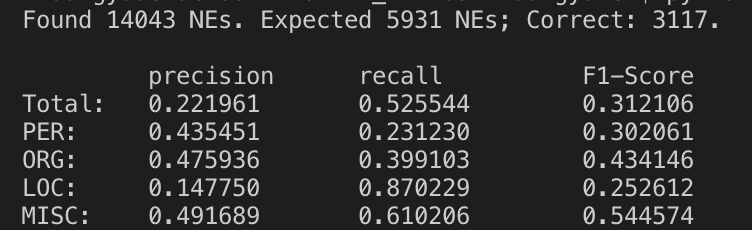
\includegraphics[scale=0.6]{42.png}\\
As we count all the words whose frequency less than 5 as '\_RARE\_', we assume all these words are of the same type. Acturally, they are not in the same type. So this way of dealing with low-frequency words is not accurate, and the percision rate is very low.\\



\section*{Question 5}
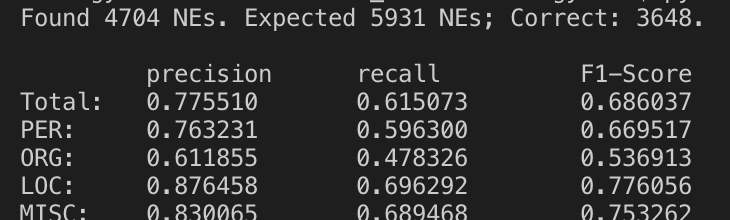
\includegraphics[scale=0.6]{52.png}\\
Using the Viterbi algorithm and counting into the context, we can see a big improvement in the accuracy.




\section*{Question 6}
I still choose the words according to their frequency.\\
If the word's frequency is less than 5, and it is s capitalized word, then I give it a new name "\_PROPER\_NAME\_".\\
If the word's frequency is less than 5, and it contains only capital letters and dots, then I give them a new name "\_FIRST\_NAME\_".\\
If the word's frequency is less than 5, and it consists only of numerals, then I give them a new name "\_NUMBER\_".\\
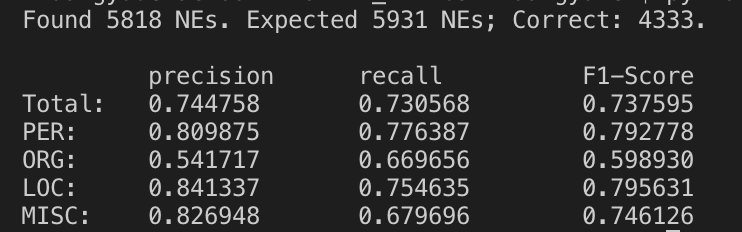
\includegraphics[scale=0.6]{6.png}\\
Now the accuracy has improved by about 5%.


% --------------------------------------------------------------
%     You don't have to mess with anything below this line.
% --------------------------------------------------------------
\end{document}
